\documentclass[conference]{IEEEtran}
\usepackage{graphicx}
\usepackage{amsmath}
\usepackage{amssymb}
\usepackage{booktabs}
\usepackage{cite}
\usepackage{array}
\usepackage{multirow}
\usepackage{url}
\usepackage{subcaption}
\usepackage{algorithm}
\usepackage{algorithmic}
\usepackage[acronym,nomain,nonumberlist]{glossaries}

% Hyperlinks are deliberately not activated: hyperref is not loaded.
\makeglossaries
\renewcommand*{\glossarysection}[2][]{}
\setglossarystyle{list}

\newacronym{bmu}{BMU}{best matching unit}
\newacronym{iqr}{IQR}{interquartile range}
\newacronym{knn}{KNN}{k-nearest neighbours}
\newacronym{qe}{QE}{quantisation error}
\newacronym{rf}{RF}{random forest}
\newacronym{som}{SOM}{self-organising map}
\newacronym{te}{TE}{topographic error}

\newcommand{\vect}[1]{\mathbf{#1}}

\title{Prediction of Cyberattacks Using Self-Organising Maps:\\
A Comparison with k-Nearest Neighbours and Random Forests}

\author{
    \IEEEauthorblockN{M Tashreeq Hartogh}
    \IEEEauthorblockA{
        27163245\\
        Department of Computer Science\\
        Stellenbosch University\\
        Stellenbosch, South Africa\\
        https://github.com/calebwidogast96-art/Unsupervised-SOM.git
    }
}

\begin{document}

\maketitle

\begin{abstract}
This report investigates the prediction of cyberattack categories from network traffic
using a \gls{som}. The UNSW-NB15 dataset contained 10 classes with a highly skewed distribution.
Preprocessing imputed missing values and transformed the numeric features.
One-hot encoding converted the nominal features.
A grid search over 480 configurations tuned five hyperparameters of the map.
The \gls{qe} served as tuning criteria.
Each neuron of the selected map received the majority class of the training instances mapped to the neuron.
The map was compared with \gls{knn} and \gls{rf} classifiers.
Both classifiers were tuned using stratified five-fold cross-validation with the macro-averaged F-measure.
The map obtained an accuracy of 0.776 on a held-out set of 51,535 instances.
The balanced accuracy was 0.418, and the macro-averaged F-measure was 0.416.
The macro-averaged F-measure of \gls{knn} was 0.526.
The value of \gls{rf} was 0.560.
The map failed to identify three minority categories.
Selection of the map using the \gls{qe} alone produced a map without topological order.
The supervised classifiers therefore outperformed the map on the minority classes.
\end{abstract}

\begin{IEEEkeywords}
self-organising map, cyberattack prediction, network intrusion detection, k-nearest neighbours,
random forest, UNSW-NB15
\end{IEEEkeywords}

\glsresetall

% ============================================================
% INTRODUCTION
% ============================================================

\section{Introduction}
\label{sec:introduction}

This section introduces the problem of cyberattack prediction and the approach followed in the report.
Section~\ref{sub:motivation} presents the motivation.
Section~\ref{sub:objectives} states the objectives.
Section~\ref{sub:structure} outlines the structure of the report.

\subsection{Motivation}
\label{sub:motivation}

Cyberattacks threaten the security of networked systems.
Intrusion detection systems monitor network traffic and raise an alert when the traffic deviates from normal behaviour.
Machine learning models learn the characteristics of malicious traffic from recorded examples.
Moustafa and Slay created the UNSW-NB15 dataset to support the evaluation of such models~\cite{Moustafa2015}.

Supervised classifiers require a label for every training instance.
Unsupervised learning discovers structure in data without labels.
The \gls{som} is an unsupervised neural network.
The network projects high-dimensional data onto a low-dimensional grid of neurons.
Similar instances activate neurons that are close on the grid.
Labelled instances then assign attack categories to the neurons.
The labelled map classifies new traffic.

The \gls{knn} classifier and the \gls{rf} classifier serve as baselines in the report.
The \gls{knn} classifier is distance based, like the \gls{som}.
The \gls{rf} classifier does not depend on the scale of the features~\cite{Hastie2009}.
The dataset poses four difficulties.
Missing values occur in several features.
Many features are strongly correlated.
Many features contain large outliers.
The class distribution is highly skewed.

\subsection{Objectives}
\label{sub:objectives}

The report pursues the following objectives.

\begin{enumerate}
    \item Apply data transformations that address the quality issues of the dataset.
    \item Tune a \gls{som} with justified optimisation procedures.
    \item Label the neurons of the trained map with cyberattack categories.
    \item Evaluate the map on instances that were not used during training or tuning.
    \item Compare the results with the \gls{knn} and \gls{rf} classifiers.
\end{enumerate}

\subsection{Report Structure}
\label{sub:structure}

The remainder of the report is organised as follows.
Section~\ref{sec:background} presents the theoretical background.
Section~\ref{sec:implementation} describes the implementation.
Section~\ref{sec:empirical} documents the empirical process.
Section~\ref{sec:results} presents and discusses the results.
Section~\ref{sec:conclusions} concludes the report.
Appendix~A lists the acronyms.

% ============================================================
% BACKGROUND
% ============================================================

\section{Background}
\label{sec:background}

This section presents the background required to follow the remainder of the report.
Section~\ref{sub:unsw} describes the dataset.
Section~\ref{sub:som} explains the \gls{som}.
Section~\ref{sub:labelling} discusses the labelling of neurons for classification.
Section~\ref{sub:knn} and Section~\ref{sub:rf} describe the two comparison classifiers.
Section~\ref{sub:preproc} covers data preprocessing.
Section~\ref{sub:measures} defines the performance measures.
Section~\ref{sub:tuning} discusses hyperparameter optimisation.

\subsection{The Dataset}
\label{sub:unsw}

The dataset is derived from the UNSW-NB15 network intrusion detection dataset
and contains network traffic features describing communication protocols,
connection states, packet statistics, data transfer rates, timing
characteristics, and connection-level behaviour. It also includes aggregated
connection counts and service-specific indicators that may help identify
suspicious activity. The $attack_cat$ attribute provides the attack category
label, enabling supervised classification of network traffic into different
attack types. These features make the dataset suitable for evaluating machine
learning approaches to network intrusion detection. The dataset is available
from the University of New South Wales website.\footnote{\url{https://research.unsw.edu.au/projects/unsw-nb15-dataset}}

\subsection{Self-Organising Maps}
\label{sub:som}
\subsubsection{Architecture and Competitive Learning}

A \gls{som} consists of $m$ neurons arranged on a regular grid.
The input space has dimension $d$.
Neuron $j$ has a fixed grid position $\vect{r}_j$ and a weight vector $\vect{w}_j$ in the input space.
The set of all weight vectors forms the codebook.
Each weight vector acts as a prototype for a region of the input space.

Training presents an instance $\vect{x}$ to the map.
The neurons compete, and the neuron with the closest weight vector wins.
The winner is the \gls{bmu}.
The index $c$ of the \gls{bmu} follows from
\begin{equation}
c = \arg\min_{j} \lVert \vect{x} - \vect{w}_j \rVert ,
\label{eq:bmu}
\end{equation}
where $\lVert \cdot \rVert$ denotes the Euclidean norm.
The weight vectors then move towards the instance according to
\begin{equation}
\vect{w}_j(t+1) = \vect{w}_j(t) + \eta(t)\, h_{cj}(t)\, \bigl(\vect{x} - \vect{w}_j(t)\bigr) .
\label{eq:update}
\end{equation}
The symbol $t$ denotes the iteration index.
The symbol $\eta(t)$ denotes the learning rate.
The function $h_{cj}(t)$ is the neighbourhood function between the winner $c$ and neuron $j$.

\subsubsection{Neighbourhood Functions}

The neighbourhood function determines the neurons that move together with the winner.
The function depends on the grid distance $\lVert \vect{r}_c - \vect{r}_j \rVert$ and on the neighbourhood width $\sigma(t)$.
The Gaussian function is
\begin{equation}
h_{cj}(t) = \exp\!\left( -\frac{\lVert \vect{r}_c - \vect{r}_j \rVert^{2}}{2\,\sigma(t)^{2}} \right) .
\label{eq:gaussian}
\end{equation}
The Gaussian function decreases smoothly with the grid distance.
The Mexican hat function is
\begin{equation}
\begin{split}
h_{cj}(t) = {} & \left( 1 - \frac{\lVert \vect{r}_c - \vect{r}_j \rVert^{2}}{\sigma(t)^{2}} \right) \\
& \times \exp\!\left( -\frac{\lVert \vect{r}_c - \vect{r}_j \rVert^{2}}{2\,\sigma(t)^{2}} \right) .
\end{split}
\label{eq:mexican}
\end{equation}
The Mexican hat function is negative for grid distances larger than $\sigma(t)$.
Neurons at these distances therefore move away from the instance.
The bubble function takes the value one for neurons within the width of the winner and zero elsewhere.
Kohonen described a neighbourhood that shrinks to the winner alone as the limit case of the algorithm~\cite{Kohonen2001}.
The limit case reduces the map to a winner-take-all vector quantiser.

\subsubsection{Training Parameters}

The learning rate and the neighbourhood width decrease during training.
Kohonen described a first phase of large neighbourhoods that orders the map.
A second phase of small neighbourhoods then fine-tunes the weight vectors~\cite{Kohonen2001}.
The asymptotic decay schedule is
\begin{equation}
\eta(t) = \frac{\eta_0}{1 + 2t/\tau} , \qquad \sigma(t) = \frac{\sigma_0}{1 + 2t/\tau} .
\label{eq:decay}
\end{equation}
The symbols $\eta_0$ and $\sigma_0$ denote the initial learning rate and the initial neighbourhood width.
The symbol $\tau$ denotes the total number of iterations.

The grid topology defines the neighbours of a neuron.
A rectangular grid places the neurons at the corners of squares.
A hexagonal grid gives each neuron six equidistant neighbours.
The side length $\lambda$ of a square map determines the number of neurons $m = \lambda^{2}$.

\subsubsection{Quality Measures}

Two measures assess a trained map.
The \gls{qe} measures how well the weight vectors represent the instances.
The \gls{qe} is
\begin{equation}
q = \frac{1}{n} \sum_{i=1}^{n} \lVert \vect{x}_i - \vect{w}_{c_i} \rVert ,
\label{eq:qe}
\end{equation}
where $n$ is the number of instances.
The vector $\vect{x}_i$ is instance $i$.
The index $c_i$ identifies the \gls{bmu} of instance $i$.

The \gls{te} measures the preservation of the grid topology.
The \gls{te} is
\begin{equation}
\begin{split}
\epsilon = \frac{1}{n} \sum_{i=1}^{n} \delta\bigl( & \text{the two best matching units} \\
& \text{of } \vect{x}_i \text{ are not adjacent} \bigr) ,
\end{split}
\label{eq:te}
\end{equation}
where $\delta(\cdot)$ equals one if the enclosed statement is true and zero otherwise.
A value of zero indicates perfect preservation, and a value of one indicates no preservation.
The two measures describe different properties.
A map therefore requires both measures for an assessment.

\subsection{Neuron Labelling for Classification}
\label{sub:labelling}

A \gls{som} is trained without labels.
Classification therefore requires a labelling step.
Each labelled training instance is presented to the map, and the label is recorded at the \gls{bmu}.
Majority voting assigns each neuron the most frequent label recorded at the neuron.
The majority label minimises the number of misclassified training instances at the neuron.

Unlabelled neurons require a fallback rule.
One rule assigns the label of the nearest labelled neuron in the input space.

The number of weight vectors is far smaller than the number of instances.
Each cluster of neurons then receives one label.
Without the clustering step, every neuron forms a separate cluster.

\subsection{k-Nearest Neighbours}
\label{sub:knn}

The classifier stores all training instances.
A new instance receives the most frequent label among the $k$ closest training instances.
The Minkowski distance between instances $\vect{x}$ and $\vect{x}'$ is
\begin{equation}
\rho(\vect{x}, \vect{x}') = \Bigl( \sum_{l=1}^{d} \lvert x_l - x'_l \rvert^{p} \Bigr)^{1/p} ,
\label{eq:minkowski}
\end{equation}
where $x_l$ is component $l$ of the vector $\vect{x}$.
The parameter $p$ defines the order of the distance.
The value $p = 1$ gives the Manhattan distance, and $p = 2$ gives the Euclidean distance.

Distance weighting gives closer neighbours more influence.
Features with large ranges dominate the distance.
Feature scaling is therefore necessary~\cite{Hastie2009}.

\subsection{Random Forests}
\label{sub:rf}

A decision tree partitions the input space recursively.
Each internal node tests one feature against a threshold.
The tree selects the split with the largest reduction in impurity.
The Gini impurity of a node is
\begin{equation}
\gamma = 1 - \sum_{y \in Y} o_y^{2} ,
\label{eq:gini}
\end{equation}
where $Y$ is the set of class labels.
The symbol $o_y$ denotes the proportion of instances of class $y$ in the node~\cite{Hastie2009}.

Each tree is trained on a bootstrap sample of the training.
Each split considers only a random subset of the features.
The forest predicts the class with the most votes.
The predicted label $\hat{y}$ of an instance $\vect{x}$ is
\begin{equation}
\hat{y} = \arg\max_{y \in Y} \sum_{b=1}^{\nu} \delta\bigl( \phi_b(\vect{x}) = y \bigr) ,
\label{eq:forest}
\end{equation}
where $\phi_b$ is the decision tree with index $b$.

Five hyperparameters control the forest.

\begin{itemize}
    \item The number of trees.
    \item The maximum depth of a tree.
    \item The minimum number of instances required to split a node.
    \item The minimum number of instances in a leaf.
    \item The number of features considered at each split.
\end{itemize}

Class weights increase the influence of minority classes during the construction of the trees.
Decision trees are invariant to monotone transformations of the features~\cite{Hastie2009}.

\subsection{Data Preprocessing}
\label{sub:preproc}
To address the known issues with the dataset, the following is performed on the data.
Imputation replaces missing values.
The median replaces missing numeric values, and the median is insensitive to outliers.
The most frequent category replaces missing nominal values.

As distance-based methods require numeric inputs of comparable scale.
The signed logarithm compresses large magnitudes and preserves the sign and zero.
The signed logarithm is
\begin{equation}
s' = \operatorname{sgn}(s)\, \ln\bigl(1 + \lvert s \rvert\bigr) ,
\label{eq:slog}
\end{equation}
where $s$ is a feature value.
Robust scaling then centres and scales the transformed values.
The scaled value $s''$ is
\begin{equation}
s'' = \frac{s' - \mu}{\kappa} ,
\label{eq:robust}
\end{equation}
where $\mu$ is the median and $\kappa$ is the \gls{iqr} of the feature in the training data.
The median and the \gls{iqr} are insensitive to extreme values.

One-hot encoding replaces a nominal feature with a binary feature for each category in the nominal feature.
The encoding avoids an artificial order among the categories.

\subsection{Performance Measures}
\label{sub:measures}

Let $u_y$ denote the number of true positives of class $y$.
Let $v_y$ denote the number of false positives.
Let $z_y$ denote the number of false negatives.

The metrics considered are defined as follows.
\\
The precision $\alpha_y$ is
\begin{equation}
\alpha_y = \frac{u_y}{u_y + v_y} .
\label{eq:precision}
\end{equation}
The recall $\beta_y$ is
\begin{equation}
\beta_y = \frac{u_y}{u_y + z_y} .
\label{eq:recall}
\end{equation}
The F-measure $f_y$ is the harmonic mean of precision and recall:
\begin{equation}
f_y = \frac{2\, \alpha_y\, \beta_y}{\alpha_y + \beta_y} .
\label{eq:fmeasure}
\end{equation}

Accuracy is the proportion of correctly classified instances.
The majority classes dominate accuracy for skewed distributions.

The balanced accuracy equals the macro-averaged recall
\begin{equation}
\bar{\beta} = \frac{1}{g} \sum_{y \in Y} \beta_y ,
\label{eq:bacc}
\end{equation}
where $g$ is the number of classes.
The macro-averaged F-measure is
\begin{equation}
\bar{f} = \frac{1}{g} \sum_{y \in Y} f_y .
\label{eq:macrof}
\end{equation}
Macro-averaging gives each class the same weight.
The weighted F-measure weights each $f_y$ by the number of instances of class $y$.

\subsection{Hyperparameter Optimisation}
\label{sub:tuning}

Grid search evaluates every combination of hyperparameter values in a predefined grid.

Cross-validation estimates the performance of a configuration on unseen data.
Stratified cross-validation was used in the optimisation step since it preserves the class proportions in every fold.
A \gls{som} is trained without labels thus labels cannot drive the tuning of a \gls{som}.
The \gls{qe} and the \gls{te} serve as unsupervised tuning criteria.

% ============================================================
% IMPLEMENTATION
% ============================================================

\section{Implementation}
\label{sec:implementation}

This section describes the implementation of the three models.
Section~\ref{sub:software} lists the software.
Section~\ref{sub:pipeline} describes the preprocessing pipelines.
Section~\ref{sub:somimpl} describes the \gls{som} implementation.
Section~\ref{sub:labelimpl} presents the algorithms for neuron labelling and class prediction.
Section~\ref{sub:clfimpl} describes the \gls{knn} and \gls{rf} implementations.

\subsection{Software}
\label{sub:software}

The implementation uses Python.
The library $scikit-learn$ provides the preprocessing and the classifiers.
The library also provides the cross-validation and the performance measures.
The library $MiniSom$ provides the \gls{som}.\footnote{\url{https://github.com/JustGlowing/minisom}}
The libraries $pandas$ and $NumPy$ handle the data.
The library $joblib$ stores the trained models.

\subsection{Preprocessing Pipelines}
\label{sub:pipeline}

A column transformer applies separate pipelines to the numeric and the nominal features.
Table~\ref{tab:pipeline} lists the steps of each model.
The \gls{som} and the \gls{knn} classifier use the same numeric pipeline.
The numeric pipeline consists of the three steps median imputation, signed logarithm ~\eqref{eq:slog} and
robust scaling ~\eqref{eq:robust}.
The \gls{rf} classifier uses median imputation only.
The nominal pipeline consists of most frequent imputation and one-hot encoding.
The encoder ignores categories that are unknown at prediction time.
The encoder produces a dense output for the \gls{som} and a sparse output for the other models.

\begin{table}[H]
\centering
\caption{Preprocessing steps of each model}
\label{tab:pipeline}
\footnotesize
\setlength{\tabcolsep}{3pt}
\begin{tabular}{lccc}
\toprule
\textbf{Step} & \shortstack{\textbf{Self-}\\\textbf{organising}\\\textbf{map}} & \shortstack{\textbf{k-nearest}\\\textbf{neighbours}} & \shortstack{\textbf{Random}\\\textbf{forest}} \\
\midrule
Numeric median imputation & Yes & Yes & Yes \\
Signed logarithm & Yes & Yes & No \\
Robust scaling & Yes & Yes & No \\
Nominal modal imputation & Yes & Yes & Yes \\
One-hot encoding & Dense & Sparse & Sparse \\
\bottomrule
\end{tabular}
\end{table}

\subsection{Self-Organising Map}
\label{sub:somimpl}

The MiniSom class implements a square map of side length $\lambda$.
The constructor receives the dimensions of the map and the hyperparameters of the training.
The initial weight vectors are randomly selected training instances.
Each training iteration draws one instance at random from the training data.
The library applies the asymptotic decay of Equation~\eqref{eq:decay} to the learning rate and to the neighbourhood width.

The Gaussian and the Mexican hat functions of MiniSom follow Equation~\eqref{eq:gaussian} and Equation~\eqref{eq:mexican}.
The bubble function of MiniSom selects the neurons whose grid coordinates differ from the coordinates of the winner by less than $\sigma(t)$ along both axes.
The comparison uses grid indices only.
The topology therefore does not influence the bubble function.
The comparison is strict.
A width of $\sigma(t) \leq 1$ therefore selects the winner alone.

The library computes the \gls{qe} of Equation~\eqref{eq:qe} and the \gls{te} of Equation~\eqref{eq:te}.
The \gls{te} counts an instance as an error if the two best matching units are not adjacent on the grid.

\subsection{Neuron Labelling and Class Prediction}
\label{sub:labelimpl}

Algorithm~\ref{alg:label} labels the neurons of a trained map.
The algorithm processes the labelled training instances once.
The labelling follows the majority vote of Section~\ref{sub:labelling}.

\begin{algorithm}[!t]
\caption{Neuron labelling}
\label{alg:label}
\begin{algorithmic}[1]
\REQUIRE A trained map and the labelled training instances.
\STATE Create an empty list of labels for every neuron.
\FOR{each training instance}
    \STATE Determine the best matching unit of the instance.
    \STATE Append the label of the instance to the list of the best matching unit.
\ENDFOR
\FOR{each neuron with a non-empty list}
    \STATE Assign the most frequent label of the list to the neuron.
\ENDFOR
\end{algorithmic}
\end{algorithm}

Algorithm~\ref{alg:predict} predicts the class of an instance.
The fallback rule of the algorithm handles best matching units without a label.

\begin{algorithm}[!t]
\caption{Class prediction}
\label{alg:predict}
\begin{algorithmic}[1]
\REQUIRE A labelled map and an instance.
\STATE Determine the best matching unit of the instance.
\IF{the best matching unit has a label}
    \STATE Return the label of the best matching unit.
\ELSE
    \STATE Compute the Euclidean distance between the instance and the weight vector of every labelled neuron.
    \STATE Return the label of the labelled neuron with the smallest distance.
\ENDIF
\end{algorithmic}
\end{algorithm}

\subsection{k-Nearest Neighbours and Random Forest}
\label{sub:clfimpl}

The scikit-learn classes \texttt{KNeighborsClassifier} and \texttt{RandomForestClassifier} implement the two baselines.
A pipeline combines the preprocessor and the classifier of each model.
Information from the validation fold therefore does not leak into the preprocessing.

The \gls{rf} classifier uses balanced class weights.
The weight of a class is inversely proportional to the frequency of the class in the training data.
The random seed of the \gls{rf} classifier is fixed at $1234$.
After the grid search, the best pipeline is refitted on the complete training set.

% ============================================================
% EMPIRICAL PROCESS
% ============================================================

\section{Empirical Process}
\label{sec:empirical}

This section documents the empirical process followed in the study.
Section~\ref{sub:data} describes the dataset.
Section~\ref{sub:prep} describes the data preparation.
Section~\ref{sub:somtune} documents the optimisation of the \gls{som}.
Section~\ref{sub:labelproc} documents the assignment of classes to neurons.
Section~\ref{sub:clftune} documents the optimisation of the comparison classifiers.
Section~\ref{sub:evalproc} describes the evaluation protocol.

\subsection{Dataset}
\label{sub:data}

The study used the file \texttt{networkTraffic.csv}.
The file contained an altered version of the UNSW-NB15 dataset.
The following data quality issues remained in the file.

\begin{itemize}
    \item Missing values were indicated by the symbol ``?''.
    \item The feature \texttt{service} contained many missing values.
    \item The feature \texttt{id} had a unique value for every instance.
    \item The features \texttt{sbytes} and \texttt{sloss} were perfectly correlated.
    \item The features \texttt{dbytes} and \texttt{dloss} were perfectly correlated.
    \item The features \texttt{is\_ftp\_login} and \texttt{ct\_ftp\_cmd} were perfectly correlated.
    \item Many other features were strongly correlated.
    \item Many features contained large positive outliers.
    \item The numeric ranges of the features differed significantly.
\end{itemize}

The three nominal features features were \texttt{proto}, \texttt{state}, and \texttt{service}.
All other features were numeric.
The target feature \texttt{attack\_cat} contained the integers zero to nine.
The mapping from integers to category names in Table~\ref{tab:classes} follows from the correspondence.
The table shows that the class distribution was highly skewed.
The largest class contained 531 times more instances than the smallest class.
The three largest classes formed 76.2\% of the evaluation set.

\begin{table}[H]
\centering
\caption{Class distribution of the evaluation set}
\label{tab:classes}
\footnotesize
\begin{tabular}{clrr}
\toprule
\textbf{Class} & \textbf{Category} & \textbf{Instances} & \textbf{Share in percent} \\
\midrule
0 & 18,600 & 36.09 \\
1 & 2,798 & 5.43 \\
2 & 466 & 0.90 \\
3 & 3,271 & 6.35 \\
4 & 8,905 & 17.28 \\
5 & 535 & 1.04 \\
6 & 4,849 & 9.41 \\
7 & 35 & 0.07 \\
8 & 302 & 0.59 \\
9 & 11,774 & 22.85 \\
\bottomrule
\end{tabular}
\end{table}

\subsection{Data Preparation}
\label{sub:prep}

\subsubsection{Cleaning of the Data}

Instances without a value for the target feature were excluded.
The feature \texttt{id} was removed.
A unique value per instance carries no information for the classification of new instances.
The second feature of each perfectly correlated pair was removed.
The removed features were \texttt{sloss}, \texttt{dloss}, and \texttt{ct\_ftp\_cmd}.
Perfect correlation makes the second feature redundant.
Redundant features also double the weight of the shared information in a distance computation.
The remaining data contained 39 features.
The features comprised 36 numeric features and three nominal features.
The other strong correlations were retained.

\subsubsection{Partitioning of the Data}

A stratified hold-out partition split the data into a training set and an evaluation set.
The evaluation set contained 20\% of the instances.
The evaluation set therefore contained 51,535 instances.
The training set contained the remaining 206,138 instances.

A stratified random subset of the training set served for hyperparameter tuning.
The subset contained 20\% of the training set.
The subset therefore contained approximately 41,200 instances.
The random seed was 1234.
The subset reduced the computational cost of tuning.

\subsubsection{Transformation of the Features}

The transformation followed the pipelines of Table~\ref{tab:pipeline}.
The median is insensitive to the large outliers.
The median therefore replaced missing numeric values.
The most frequent category replaced the missing values of \texttt{service}.
The signed logarithm reduced the influence of the large positive outliers.
Robust scaling brought the numeric ranges to a comparable scale.
One-hot encoding converted the nominal features to numeric features.
Since decision trees are invariant to monotone transformations the \gls{rf} classifier
therefore received no transformation of the numeric features.

The preprocessor was fitted on training data only.
The evaluation data were transformed using the fitted parameters.
The preprocessor of the \gls{som} was fitted on the complete training set before the tuning subset was drawn.
The preprocessors of the \gls{knn} and \gls{rf} classifiers were fitted inside each cross-validation fold.

\subsection{Hyperparameter Optimisation of the Self-Organising Map}
\label{sub:somtune}

The tuning used a grid search over five hyperparameters.
Table~\ref{tab:grids} lists the values.
The grid contained $5 \times 4 \times 4 \times 3 \times 2 = 480$ configurations.
Every configuration was trained for 30,000 iterations on the tuning subset.
The random seed 1234 initialised the random number generator of every map.

\begin{table*}[!t]
\centering
\caption{Hyperparameter grids of the three models}
\label{tab:grids}
\footnotesize
\begin{tabular}{llp{9.5cm}}
\toprule
\textbf{Model} & \textbf{Hyperparameter} & \textbf{Values} \\
\midrule
\multirow{5}{*}{Self-organising map} & Side length $\lambda$ & 10, 15, 20, 25, 30 \\
 & Initial learning rate $\eta_0$ & 0.1, 0.3, 0.5, 0.7 \\
 & Initial neighbourhood width $\sigma_0$ & 1, 2, 3, 5 \\
 & Neighbourhood function & Gaussian, Mexican hat, bubble \\
 & Topology & Rectangular, hexagonal \\
\midrule
\multirow{4}{*}{k-nearest neighbours} & Number of neighbours $k$ & 3, 5, 7, 9, 11, 15 \\
 & Weighting & Uniform, distance \\
 & Distance order $p$ & 1, 2 \\
 & Leaf size & 20, 30, 40 \\
\midrule
\multirow{5}{*}{Random forest} & Number of trees $\nu$ & 100, 200, 300 \\
 & Maximum depth & Unbounded, 10, 20 \\
 & Minimum instances to split & 2, 10 \\
 & Minimum instances per leaf & 2, 5 \\
 & Features per split & Square root, base-two logarithm \\
\bottomrule
\end{tabular}
\end{table*}

The ranges followed four considerations.
The side lengths gave maps of 100 to 900 neurons.
The Vesanto rule of thumb gave approximately 1,015 neurons for 41,200 instances.
The largest map therefore approached the recommended size.
The initial neighbourhood widths covered a narrow neighbourhood and a neighbourhood that spanned half of the smallest map.
The learning rates covered slow and fast adaptation.
The three neighbourhood functions and the two topologies covered the options of the library.

The criteria were the \gls{qe} and the \gls{te}.
Both were computed on the tuning subset.
The selection rule chose the configuration with the lowest \gls{qe}.
The configurations were evaluated in the order of the grid, and the rectangular topology preceded the hexagonal topology.
A later configuration replaced the selected configuration only if the \gls{qe} was strictly lower.

Configurations with an infinite or undefined \gls{qe} were never selected.
The tuning log recorded the numeric hyperparameters and the two criteria.
The log also recorded the training time.

\subsection{Assignment of Classes to Neurons}
\label{sub:labelproc}

The selected map was labelled with Algorithm~\ref{alg:label}.
The labelling used the complete training set of 206,138 instances.

Majority voting was chosen for two reasons.
First, the majority label minimises the number of misclassified training instances at a neuron.
Second, the rule requires no additional hyperparameter.
Neurons without training instances received no label.
Algorithm~\ref{alg:predict} assigned the label of the nearest labelled neuron to instances whose best matching unit had no label.
No alternative labelling strategy was evaluated.
Each neuron formed one cluster of training instances.
Further clustering on the weight vectors added additional complexity and hyperparemeters to find an appropriate clustering.
With limited resources the attemps made yielded poor results but its inconclusive as to whether this approach is worse.
It's not explored further as the original approach yielded comparable results to that of \gls{knn} and \gls{rf}, which
forms the framework of the discussion and comparisons in this report.

\subsection{Hyperparameter Optimisation of the Comparison Classifiers}
\label{sub:clftune}

Table~\ref{tab:grids} lists the grids of the \gls{knn} and \gls{rf} classifiers.
Each grid contained 72 configurations.
Stratified five-fold cross-validation evaluated each configuration on the tuning subset.
The folds were shuffled with the random seed 1234.
The tuning criterion was the macro-averaged F-measure of Equation~\eqref{eq:macrof}.
The best configuration of each classifier was refitted on the complete training set.

\subsection{Evaluation Protocol}
\label{sub:evalproc}

The evaluation set remained unused until the final prediction.
Each final model predicted the classes of the evaluation set once.
The evaluation reported the accuracy and the balanced accuracy.
The evaluation also reported the macro-averaged precision and recall.
The macro-averaged F-measure and the weighted F-measure completed the overall measures.
The three measures of every class served for the comparison per class.

% ============================================================
% RESULTS AND DISCUSSION
% ============================================================

\section{Results and Discussion}
\label{sec:results}

This section presents and discusses the results.
Section~\ref{sub:res_som} reports the tuning of the \gls{som}.
Section~\ref{sub:res_clf} reports the tuning of the comparison classifiers.
Section~\ref{sub:res_gen} reports the performance on the evaluation set.
Section~\ref{sub:res_disc} discusses the findings and the limitations.

\subsection{Tuning Results of the Self-Organising Map}
\label{sub:res_som}

\subsubsection{Overview}

All 480 configurations completed.
The \gls{qe} was infinite or undefined for 68 configurations.
The configurations formed 14.2\% of the grid.
The count increased with the initial neighbourhood width.
The count increased from 5 at a width of 1 to 26 at a width of 5.
At most two configurations diverged for each combination of the three numeric hyperparameters.
The maximum equals the number of topologies.
The divergence therefore occurred in a single neighbourhood function.
The Mexican hat function is the only evaluated function with negative values which move neurons away from the instances.
The divergence is attributed to the Mexican hat function.
The remaining 412 configurations had a \gls{qe} between 0.600 and 3.582.

\subsubsection{Effect of the Map Size}

Table~\ref{tab:size} shows the effect of the side length.
The median \gls{qe} decreased from 1.428 for the smallest maps to 0.833 for the largest maps.
Figure~\ref{fig:size} shows the decrease for every neighbourhood width.
The mean training time increased from 1.74 seconds to 13.76 seconds.
The number of neurons increased by a factor of nine, and the training time increased by a factor of 7.9.
The \gls{qe} was computed on the training data of the map.
A larger codebook represents the training data more closely.
The \gls{qe} therefore decreased with the size of the map without an interior optimum.

\begin{table}[H]
\centering
\caption{Effect of the map size on the quantisation error and the training time}
\label{tab:size}
\footnotesize
\begin{tabular}{rrrr}
\toprule
\textbf{Side length} & \textbf{Neurons} & \shortstack{\textbf{Median}\\\textbf{quantisation}\\\textbf{error}} & \shortstack{\textbf{Mean time}\\\textbf{in seconds}} \\
\midrule
10 & 100 & 1.428 & 1.74 \\
15 & 225 & 1.178 & 3.39 \\
20 & 400 & 1.016 & 6.03 \\
25 & 625 & 0.912 & 9.59 \\
30 & 900 & 0.833 & 13.76 \\
\bottomrule
\end{tabular}
\end{table}

\begin{figure*}[!t]
\centering
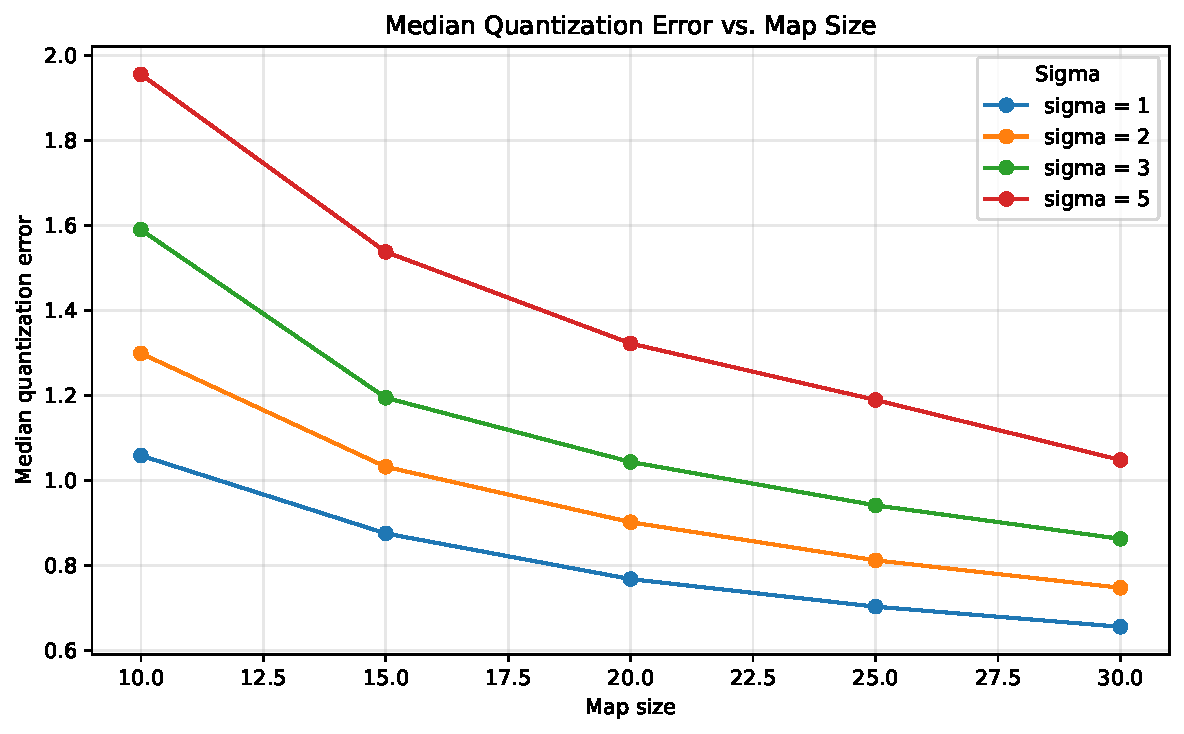
\includegraphics[width=3.4in]{figs/fig_qe_size.pdf}
\caption{Median error of the finite configurations against the map side length for four initial neighbourhood widths}
\label{fig:size}
\end{figure*}

\subsubsection{Effect of the Neighbourhood Width and the Learning Rate}

The initial neighbourhood width had opposite effects on the two criteria.
The median \gls{qe} increased from 0.866 to 1.199 as the width increased from 1 to 5.
The median \gls{te} decreased from 0.987 to 0.041.

A narrow neighbourhood gave a low \gls{qe} and a \gls{te} close to one.
A wide neighbourhood gave a \gls{te} close to zero and a higher \gls{qe}.
A total of 101 configurations had a \gls{te} above 0.9, and 190 configurations had a \gls{te} below 0.1.

The median \gls{qe} decreased from 1.130 to 1.031 when the learning rate increased from 0.1 to 0.3.
The median \gls{qe} was 1.017 and 1.024 for the learning rates 0.5 and 0.7.
The learning rate above 0.3 therefore had a negligible effect.

\subsubsection{Selected Configuration}

Table~\ref{tab:selected} lists three configurations which briefly demonstrates a trafe-off between \gls{qe} and \gls{te}.
The first row lists the configuration with the lowest \gls{qe}.
The \gls{qe} was 0.600, and the \gls{te} exceeded 0.99.
The selection rule chose the configuration.
Two alternatives are listed for comparison.
The lowest \gls{qe} among the configurations with a \gls{te} below 0.1 was 0.732.
The lowest \gls{qe} among the configurations with a \gls{te} below 0.01 was 1.457.

\begin{table}[H]
\centering
\caption{Selected configurations of the map}
\label{tab:selected}
\footnotesize
\setlength{\tabcolsep}{3pt}
\begin{tabular}{lrrrrr}
\toprule
\textbf{Criterion} & $\lambda$ & $\eta_0$ & $\sigma_0$ & \shortstack{\textbf{Quantisation}\\\textbf{error}} & \shortstack{\textbf{Topographic}\\\textbf{error}} \\
\midrule
Lowest error & 30 & 0.3 & 1 & 0.600 & $>$0.99 \\
Topographic error $<$ 0.1 & 30 & 0.5 & 2 & 0.732 & 0.073 \\
Topographic error $<$ 0.01 & 10 & 0.3 & 3 & 1.457 & 0.008 \\
\bottomrule
\end{tabular}
\end{table}

The selected configuration had a neighbourhood width of 1 and the bubble function with a rectangle topology.
Section~\ref{sub:somimpl} explained that the bubble function with a width of at most one updates the winner alone.
The selected map therefore performed winner-take-all learning without cooperation between neighbouring neurons.
The map acted as an online vector quantiser with 900 prototypes.
The \gls{te} above 0.99 confirmed the absence of topological order.
The selection by the \gls{qe} alone favoured the degenerate solution.
The side length of 30 and the neighbourhood width of 1 are also the boundary values of the grid.
Larger maps and narrower neighbourhoods were not evaluated.

\subsection{Tuning Results of the Comparison Classifiers}
\label{sub:res_clf}

Table~\ref{tab:best} lists the best configurations.
The best \gls{knn} configuration used three neighbours and the Manhattan distance.
The vote of each neighbour was weighted by the distance.
The cross-validated macro-averaged F-measure was 0.4813.
The best \gls{rf} configuration contained 300 trees of unbounded depth.
The cross-validated macro-averaged F-measure was 0.5339.

\begin{table}[H]
\centering
\caption{Best configurations of the comparison classifiers}
\label{tab:best}
\footnotesize
\setlength{\tabcolsep}{3pt}
\begin{tabular}{p{0.95in}p{1.4in}p{0.85in}}
\toprule
\textbf{Model} & \textbf{Best configuration} & \textbf{F-measure} \\
\midrule
k-nearest neighbours & $k=3$, distance weights, $p=1$, leaf size 20 & $0.4813 \pm 0.0148$ \\
Random forest & $\nu=300$, unbounded depth, split 2, leaf 2, square root & $0.5339 \pm 0.0246$ \\
\bottomrule
\end{tabular}
\end{table}

The \gls{knn} scores decreased with the number of neighbours.
The mean score over the grid was 0.4802 for three neighbours and 0.4585 for 15 neighbours.
The best value lay on the lower boundary of the grid.
The Manhattan distance gave a higher mean score than the Euclidean distance, namely 0.4708 against 0.4644.
Distance weighting gave a marginally higher mean score than uniform weighting, namely 0.4685 against 0.4667.
The three leaf sizes gave identical scores.
The leaf size therefore did not influence the predictions.
The mean scoring time per fold was 32.2 seconds for the Manhattan distance and 3.7 seconds for the Euclidean distance.

The \gls{rf} scores depended mainly on the depth.
The mean score over the grid was 0.4589 for a depth of 10.
The mean scores were 0.5067 for a depth of 20 and 0.5080 for unbounded depth.
The leaf size and the number of features had smaller effects.
The minimum leaf size of two gave 0.5015, and the leaf size of five gave 0.4809.
The square root of the number of features gave 0.5005, and the base-two logarithm gave 0.4819.
The number of trees had a negligible effect.
The mean scores varied between 0.4906 and 0.4916.
The best configuration used the smallest leaf size of the grid.
The second-best configuration used 100 trees and a depth of 20.
The score was 0.5337, and the mean fitting time was 8.4 seconds against 30.8 seconds for the best configuration.

The differences between the top configurations were small.
The ten best \gls{rf} configurations spanned 0.0065 in score.
The standard deviation over the folds of the best configuration was 0.0246.

\subsection{Performance on the Evaluation Set}
\label{sub:res_gen}

Table~\ref{tab:overall} lists the overall performance.
The \gls{knn} classifier achieved the highest accuracy of 0.796.
The \gls{som} achieved an accuracy of 0.776, and the \gls{rf} classifier achieved an accuracy of 0.748.
The ranking reversed for the balanced accuracy and the macro-averaged F-measure.
The \gls{rf} classifier achieved the highest balanced accuracy of 0.615 and the highest macro-averaged F-measure of 0.560.
The \gls{som} achieved the lowest values of 0.418 and 0.416.
The \gls{knn} classifier achieved 0.518 and 0.526.

\begin{table*}[!t]
\centering
\caption{Precision $\alpha_y$, recall $\beta_y$, and F-measure $f_y$ of every class on the evaluation set}
\label{tab:perclass}
\footnotesize
\begin{tabular}{cl | ccc | ccc | ccc}
\toprule
 & & \multicolumn{3}{c}{\textbf{k-nearest neighbours}} & \multicolumn{3}{c}{\textbf{Random forest}} & \multicolumn{3}{c}{\textbf{Self-organising map}} \\
\cmidrule(lr){3-5}\cmidrule(lr){6-8}\cmidrule(lr){9-11}
\textbf{Class} & \textbf{Class \%} & $\alpha_y$ & $\beta_y$ & $f_y$ & $\alpha_y$ & $\beta_y$ & $f_y$ & $\alpha_y$ & $\beta_y$ & $f_y$ \\
\midrule
0 & 36.09 & 0.91 & 0.92 & 0.92 & 0.98 & 0.80 & 0.88 & 0.86 & 0.90 & 0.88 \\
1 & 5.43 & 0.62 & 0.75 & 0.68 & 0.84 & 0.82 & 0.83 & 0.71 & 0.60 & 0.65 \\
2 & 0.90 & 0.06 & 0.10 & 0.08 & 0.02 & 0.20 & 0.04 & 0.00 & 0.00 & 0.00 \\
3 & 6.35 & 0.34 & 0.36 & 0.35 & 0.31 & 0.20 & 0.24 & 0.34 & 0.05 & 0.09 \\
4 & 17.28 & 0.69 & 0.68 & 0.69 & 0.86 & 0.54 & 0.66 & 0.58 & 0.88 & 0.70 \\
5 & 1.04 & 1.04 & 0.12 & 0.20 & 0.05 & 0.16 & 0.07 & 0.00 & 0.00 & 0.00 \\
6 & 9.41 & 0.65 & 0.57 & 0.61 & 0.53 & 0.82 & 0.64 & 0.53 & 0.44 & 0.48 \\
7 & 0.07 & 0.33 & 0.23 & 0.27 & 0.64 & 0.77 & 0.70 & 0.00 & 0.00 & 0.00 \\
8 & 0.59 & 0.52 & 0.47 & 0.49 & 0.39 & 0.87 & 0.54 & 0.45 & 0.34 & 0.39 \\
9 & 22.85 & 0.99 & 0.98 & 0.99 & 1.00 & 0.97 & 0.99 & 0.99 & 0.97 & 0.98 \\
\bottomrule
\end{tabular}
\end{table*}

\begin{table}[!t]
\centering
\caption{Overall performance on the evaluation set}
\label{tab:overall}
\footnotesize
\begin{tabular}{lccc}
\toprule
\textbf{Measure} & \shortstack{\textbf{k-nearest}\\\textbf{neighbours}} & \shortstack{\textbf{Random}\\\textbf{forest}} & \shortstack{\textbf{Self-}\\\textbf{organising}\\\textbf{map}} \\
\midrule
Accuracy & 0.796 & 0.748 & 0.776 \\
Balanced accuracy & 0.518 & 0.615 & 0.418 \\
Macro-averaged precision & 0.57 & 0.56 & 0.45 \\
Macro-averaged recall & 0.52 & 0.62 & 0.42 \\
Macro-averaged F-measure & 0.526 & 0.560 & 0.416 \\
Weighted F-measure & 0.80 & 0.78 & 0.75 \\
\bottomrule
\end{tabular}
\end{table}

Table~\ref{tab:perclass} lists the results of every class.
Figure~\ref{tab:perclass} compares the F-measures.
All three models classified class 9 almost perfectly with F-measures ranged from 0.98 to 0.99.
All three models achieved F-measures above 0.65 for class 4.
The models differed strongly on the minority classes.

\subsection{Discussion}
\label{sub:res_disc}

\subsubsection{Comparison of the Models}

The accuracy and the macro-averaged measures ranked the models differently.
The three largest classes formed 76.2\% of the evaluation set.
Accuracy therefore reflected the performance on the majority classes.
The macro-averaged measures reflected the performance on all classes.
The \gls{rf} classifier achieved the best macro-averaged F-measure.
The \gls{knn} classifier achieved the best accuracy.
The \gls{som} was inferior to the \gls{knn} classifier by 0.020 in accuracy and by 0.110 in the macro-averaged F-measure.
The same preprocessing was applied to both models.
The \gls{knn} classifier stored all 206,138 training instances.
The \gls{som} stored 900 prototypes.
The prototypes compress the training data by a factor of 229.

\subsubsection{Behaviour of the Random Forest and KNN}

The \gls{rf} classifier traded precision for recall.
The balanced class weights raised the recall of the minority classes.
The recall of class 8 was 0.87 for the \gls{rf} classifier and 0.47 for the \gls{knn} classifier.
The recall of class 7 was 0.77 against 0.23.
The precision decreased accordingly.
The precision of class 8 was 0.39 against 0.52.
The precision of class 5 was 0.05 against 0.60.

The recall of the class 0 was 0.80 for the \gls{rf} classifier and 0.92 for the \gls{knn} classifier.
The \gls{rf} classifier therefore misclassified about one fifth of class 0.
In an intrusion detection system false alarms impose a cost on the operators.
The precision of the class 0 was 0.98 for the \gls{rf} classifier.
A class 0 prediction of the \gls{rf} classifier was therefore reliable.

\subsubsection{Behaviour of the Self-Organising Map}

The \gls{som} classified no instance of three minority categories correctly.
The categories were class 2, class 5, and class 7 which contained 1,036 instances (2.0\% of the evaluation set)
The recall of class 3 also really low at 0.05.
The recall of the class 4 was 0.88 and the precision was 0.58 so the \gls{som} therefore predicted
approximately 13,500 instances as class 4 when the evaluation set contained 8,905 instances of the category.
The labelling explains the pattern as majority voting assigns a neuron to a minority class only if the minority
class outnumbers all other classes at the neuron.
Class 4 is the second largest class of the dataset.
The class therefore won the neurons in regions where the classes overlap.
The \gls{knn} classifier retrieved 10\% to 23\% of the instances of these three failed categories.
The information for a partial recognition was therefore present in the preprocessed features for \gls{knn}.
The 900 prototypes with majority labels did not retain the information.

The selection of the map affected the result.
The selected map performed winner-take-all learning.
The weight vectors resulted from 20\% of the training set.
The training used fewer iterations than the tuning subset had instances.
The learning algorithm therefore presented fewer than one pass of the tuning subset to the map.
No experiment isolated the contribution of each decision.
The \gls{som} results therefore document the performance of the selected configuration and not the limit of the method.

\subsubsection{Evaluation Reliability}

Class 7 contained 35 evaluation instances.
One instance changed the recall of the category by 2.9 percentage points.
The F-measures of 0.70 for the \gls{rf} classifier and 0.27 for the \gls{knn} classifier on the class are therefore uncertain.
The results of a single partition and a single run do not provide confidence intervals.
The differences between the models on the majority classes are small and require repetition for confirmation.
The differences on the three minority categories are large.


\subsubsection{Limitations}

The study had the following limitations.

\begin{itemize}
    \item The \gls{som} and the two baselines used different random partitions.
    \item The selection of the map used the \gls{qe} alone, and the grid boundaries coincided with the selected values.
    \item The \gls{qe} and the \gls{te} were computed on the training data of the map.
    \item The weight vectors resulted from the tuning subset only.
    \item Only majority voting was evaluated for the assignment of classes.
    \item The weight vectors were not clustered beyond the individual neurons.
    \item Strong correlations other than the perfect correlations were retained.
\end{itemize}

% ============================================================
% CONCLUSIONS
% ============================================================

\glsreset{som}
\glsreset{knn}
\glsreset{rf}
\glsreset{qe}
\glsreset{te}
\glsreset{bmu}

\section{Conclusions}
\label{sec:conclusions}

\subsection{Summary of Findings}

The study investigated the prediction of cyberattack categories with a \gls{som} and compared the map with \gls{knn} and \gls{rf} classifiers.
The data transformations addressed the data quality issues of the dataset.
The tuning of the \gls{som} evaluated 480 configurations using the \gls{qe} and the \gls{te}.
The selection by the \gls{qe} alone chose a map with 900 neurons and a narrow bubble neighbourhood.
The \gls{te} of the map exceeded 0.99.
The map therefore did not preserve topology.
The labelling used the majority class of the training instances at each neuron.

The \gls{som} achieved an accuracy of 0.776 and a balanced accuracy of 0.418.
The macro-averaged F-measure was 0.416.
The \gls{knn} classifier achieved a macro-averaged F-measure of 0.526.
The \gls{rf} classifier achieved a macro-averaged F-measure of 0.560.
The \gls{som} did not identify three minority categories.
The supervised classifiers therefore outperformed the \gls{som} on the minority classes.
The \gls{rf} classifier achieved the best recall of the minority classes at the cost of false alarms on class 0.

\subsection{Limitations and Future Work}

The \gls{som} and the baselines used different random partitions.
Future work should use identical partitions for all models.
The tuning should combine the \gls{qe} with the \gls{te}, or should use the classification performance on a validation set.
The grid should include larger maps and a wider range of neighbourhood widths.
The final map should train on the complete training set for more than one pass of the data.
Class-balanced voting should replace majority voting to give minority classes a chance to win neurons.
The weight vectors should be clustered with the hierarchical clustering method for \gls{som} codebook vectors.
In which each cluster should then receive a label.
Repeated partitions should provide confidence intervals for the comparison.

% ============================================================
% APPENDICES
% ============================================================

\appendices

\section{Acronyms}
\glsaddall
\printglossary[type=\acronymtype]

\section{Symbols}

The symbols are listed in alphabetical order, with Latin symbols before Greek symbols.

\begin{table}[!h]
\centering
\footnotesize
\begin{tabular}{lp{2.45in}}
\toprule
\textbf{Symbol} & \textbf{Definition} \\
\midrule
$b$ & Index of a decision tree \\
$c$, $c_i$ & Index of the best matching unit of an instance \\
$d$ & Dimension of the input space \\
$f_y$ & F-measure of class $y$ \\
$\bar{f}$ & Macro-averaged F-measure \\
$g$ & Number of classes \\
$h_{cj}$ & Neighbourhood function between neurons $c$ and $j$ \\
$i$ & Index of an instance \\
$j$ & Index of a neuron \\
$k$ & Number of neighbours \\
$l$ & Index of a feature \\
$m$ & Number of neurons \\
$n$ & Number of instances \\
$o_y$ & Proportion of class $y$ in a decision tree node \\
$p$ & Order of the Minkowski distance \\
$q$ & Quantisation error \\
$\vect{r}_j$ & Grid position of neuron $j$ \\
$s$, $s'$, $s''$ & Feature value, signed logarithm of the value, scaled value \\
$t$ & Iteration index \\
$u_y$ & Number of true positives of class $y$ \\
$v_y$ & Number of false positives of class $y$ \\
$\vect{w}_j$ & Weight vector of neuron $j$ \\
$\vect{x}$, $\vect{x}_i$ & Instance \\
$y$ & Class label \\
$\hat{y}$ & Predicted class label \\
$Y$ & Set of class labels \\
$z_y$ & Number of false negatives of class $y$ \\
$\alpha_y$ & Precision of class $y$ \\
$\beta_y$ & Recall of class $y$ \\
$\bar{\beta}$ & Balanced accuracy \\
$\gamma$ & Gini impurity \\
$\delta(\cdot)$ & Indicator function \\
$\epsilon$ & Topographic error \\
$\eta$, $\eta_0$ & Learning rate, initial learning rate \\
$\kappa$ & Interquartile range of a feature \\
$\lambda$ & Side length of a square map \\
$\mu$ & Median of a feature \\
$\nu$ & Number of decision trees \\
$\rho$ & Minkowski distance function \\
$\sigma$, $\sigma_0$ & Neighbourhood width, initial neighbourhood width \\
$\tau$ & Total number of training iterations \\
$\phi_b$ & Decision tree with index $b$ \\
\bottomrule
\end{tabular}
\end{table}

% ============================================================
% REFERENCES
% ============================================================

\begin{thebibliography}{99}

\bibitem{Breiman1996}
L. Breiman,
``Bagging predictors,''
\textit{Machine Learning}, vol. 24, no. 2, pp. 123--140, 1996.

\bibitem{Breiman2001}
L. Breiman,
``Random forests,''
\textit{Machine Learning}, vol. 45, no. 1, pp. 5--32, 2001.

\bibitem{Engelbrecht2007}
A. P. Engelbrecht,
\textit{Computational Intelligence: An Introduction}, 2nd ed.
Chichester, United Kingdom: Wiley, 2007.

\bibitem{Hastie2009}
T. Hastie, R. Tibshirani, and J. Friedman,
\textit{The Elements of Statistical Learning: Data Mining, Inference, and Prediction}, 2nd ed.
New York, United States: Springer, 2009.

\bibitem{Kohonen2001}
T. Kohonen,
\textit{Self-Organizing Maps}, 3rd ed.
Berlin, Germany: Springer, 2001.

\bibitem{Moustafa2015}
N. Moustafa and J. Slay,
``UNSW-NB15: A comprehensive data set for network intrusion detection systems,''
in \textit{Proceedings of the Military Communications and Information Systems Conference}, 2015, pp. 1--6.

\end{thebibliography}

\end{document}